%---------------------------------
% Úvod
%---------------------------------
\chapter{Úvod}
Tradičné redakčné systémy pre správu obsahu sú obvykle zostavené z~dvoch hlavných súčastí -- administračného a verejného webového rozhrania. Administračné rozhranie slúži pre vytváranie a úpravu obsahu, webové na jeho nasledné zobrazenie. Webové rozhranie je obvykle jednotné pre všetky platformy a zariadenia na ktorých je využívané, tzn. že jeho používanie je často neoptimálne. Pre tento dôvod sa začali využívať systémy bez webového rozhrania disponujúce klasickým administračným rozhraním a otvoreným aplikačným rozhraním (API\footnote{API -- Application programming interface}), umožnujúcim získavanie obsahu na požadované platformy. Tento obsah je následne možné optimalizovať individuálne podľa potreby. Súčasné riešenia redakčných systémom s~otvoreným rozhraním sú často robustné systémy, ktoré však vyžadujú komplexnú konfiguráciu predtým ako ich je možné začať využívať. Niektoré takéto systémy vyžadujú aj vlastnú infraštruktúru pre ich nasadenie. Tieto skutočnosti otvárajú priestor pre redakčný systém, ktorý by pomohol vyriešiť tieto prekážky. Takýto systém je cieľom tejto práce.

Navrhovaný systém poskytuje možnosť správy obsahu bez nutnosti úvodnej konfigurácie a infraštruktúry. Obsah je možné spravovať pomocou užívateľského rozhrania v~aplikácii Slack alebo webového rozhrania. Plnú funkcionalitu však užívateľ môže využiť bez nutnosti používania webového rozhrania.

\subsection*{Obsah kapitol}
Prvá kapitola, \nameref{chapter:theory}, sa skladá zo~štyroch sekcií venovaným postupne existujúcim riešeniam podobným tejto práci, vývoji serverových aplikácii, klientských aplikácii a~špecifikácii GraphQL.

% TODO: Add introduction to document's structure.

%---------------------------------
% Teoretická časť
%---------------------------------
\chapter{Teoretická časť}
\label{chapter:theory}
Správa obsahu a jeho doručenie konzumentom. Táto kapitola popisuje základné princípy, techniky a technológie, ktoré sú nutné pre zostavenie a pochopenie princípu fungovania tejto práce.

\section{Redakčné systémy s~otvoreným aplikačným rozhraním}
Redakčné systémy disponujúce iba skrytou administračnou časťou a verejným aplikačným rozhraním sú typicky nazývané \textbf{headless}\footnote{headless -- ang. bez hlavy (bez webového rozhrania)} redakčné systémy. Tieto riešenia štandardne disponujú rozhraním REST\footnote{REST -- Representational State Transfer} alebo GraphQL, ktoré implementuje aj táto práca. Headless redakčný systém nerieši zobrazenie samotného obsahu. Jediný spôsob ako obsah získať je využiť niektoré z~dostupných rozhraní poskytované konkrétnym riešením. Výhodou oproti tradičným redakčným systémom je možnosť získané dáta optimalizovane zobraziť na rôznych zariadeniach. 

\begin{figure}[h]
	\centering
	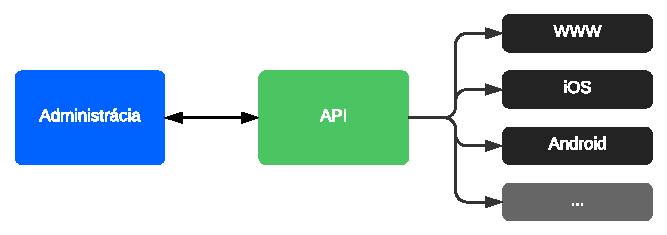
\includegraphics{obrazky-figures/headless_cms_graph.pdf}
	\caption{Ilustračná schéma generického headless redakčného systému.}
\end{figure}

Členenie obsahu v~takýchto redakčných systémoch je typicky v~dvoch vrstvách -- kategórie a obsahové typy (komponenty). Kategórie sú zoznamy združujúce jednotlivé komponenty, môžu byť homogénne (všetky prvky zoznamu sú jednoho typu) alebo heterogénne (prvky zoznamu sú typicky iných typov). Komponenty sú atomickými prvkami headless redakčných systémov. Môžu nadobúdať rôznych typov, ktoré určujú ich vnútornú dátovú štruktúru. Typický príklad často používaných typov komponentov sú napríklad \texttt{prostý text} alebo \texttt{odkaz}. Niektoré headless redakčné systémy umožňujú vytvárať aj vlastné typy komponentov a tak si prospôsobiť dáta vlastným špecifickým potrebám.

\subsection{Strapi}
\blockquote[Dokumentácia Strapi.io \cite{StrapiDocs}]{Strapi je flexibilný, open-source\footnote{open-source -- otvorený kód, zväčša vyvíjaný komunitou} Headless CMS\footnote{CMS -- ang. content management system (redakčný systém)}, ktorý dáva vývojárom slobodu voľby ich obľúbených nástrojov a zároveň dovoľuje editorom jednoducho spravovať a distribuovať ich obsah.}

\bigskip

Najpopulárnejší Headless redakčný systém. Disponuje administračným panelom zostaveným namieru, REST aj GraphQL rozhraním, systémom uživateľských práv a mnohými inými vlastnosťami. Tento redakčný systém má aj obchod s aplikáciami, ktoré si môžu používateľia pridať a tým rozšíriť funkcionalitu. 

\bigskip

\lstset{style=codestyle}

\begin{lstlisting}[caption=Príklad HTTP požiadavku na REST rozhranie Strapi]
	GET http://localhost:1337/restaurants/count
\end{lstlisting}

\bigskip

Pre použitie Strapi je nutné systém spustiť na vlastnej infraštruknúre, pripojiť k predom vytvorenej relačnej databáze a celý systém nakonfigurovať.

\subsection{Netlify CMS}
\blockquote[Dokumentácia Netlify CMS \cite{NetlifyDocs}]{Netlify CMS je open-source content management systém, ktorý pre ukladanie dát využíva Git repozitáre. Jadro Netlify CMS tvorí React aplikácia ktorá využíva rozhranie pre prácu s GitHub\footnote{\href{https://developer.github.com/v3/}{https://developer.github.com/v3/}}, GitLab\footnote{\href{https://docs.gitlab.com/ee/api/}{https://docs.gitlab.com/ee/api/}} alebo Bitbucket\footnote{\href{https://confluence.atlassian.com/bitbucket/rest-apis-222724129.html}{https://confluence.atlassian.com/bitbucket/rest-apis-222724129.html}} API.}

\section{Vývoj serverových aplikácii}
\texttt{Server} -- centrálny počítač z ktorého ostatné počítače získavajú informácie. \cite{CamDict} \\

\noindent Serverová aplikácia je proces spustený na centrálne dostupnom zariadení. Obvykle slúži ako zdroj informácií pre ostatné zariadenia, typicky v počítačovej sieti. Tento proces očakáva požiadavky a odpovedá na ne vopred určenou reakciou. Serverové aplikácie je možné implementovať v rôznych programovacích jazykoch, no medzi najpoužívanejšie patrí PHP, Java, Python alebo JavaScript (popr. rozšírenie TypeScript). Aplikácia má ďaľej určený komunikačný protokol, pomocou ktorého prijíma požiadavky a odosiela odpovede. Pri bežných aplikáciach ide najčastejšie protokol HTTP.

\subsection{TypeScript}
TypeScript je rozšírenie programovacieho jazyka JavaScript. Jedná sa o silne typovaný, objektovo orientovaný a kompilovaný programovací jazyk \cite{TSWeb}. TypeScript je obvykle nutné skompilovať do natívneho JavaScriptu pre zachovanie kompatibility. Využívanie TypeScriptu nie je nutné, avšak vďaka vlastnosti silného typovania umožní vývojárovi predísť chybám ešte pred kompiláciou.
 
\section{Vývoj klientských aplikácii}
\section{GraphQL}
